% !TEX root = ../../1-te.tex
\tocheck{4}{Aktuelle Musterstudienpläne der FG beschaffen (abängig von der BPO!) und einfügen
}
\label{musterstudienplan}
\iftoggle{winter}{
	\begin{center}
		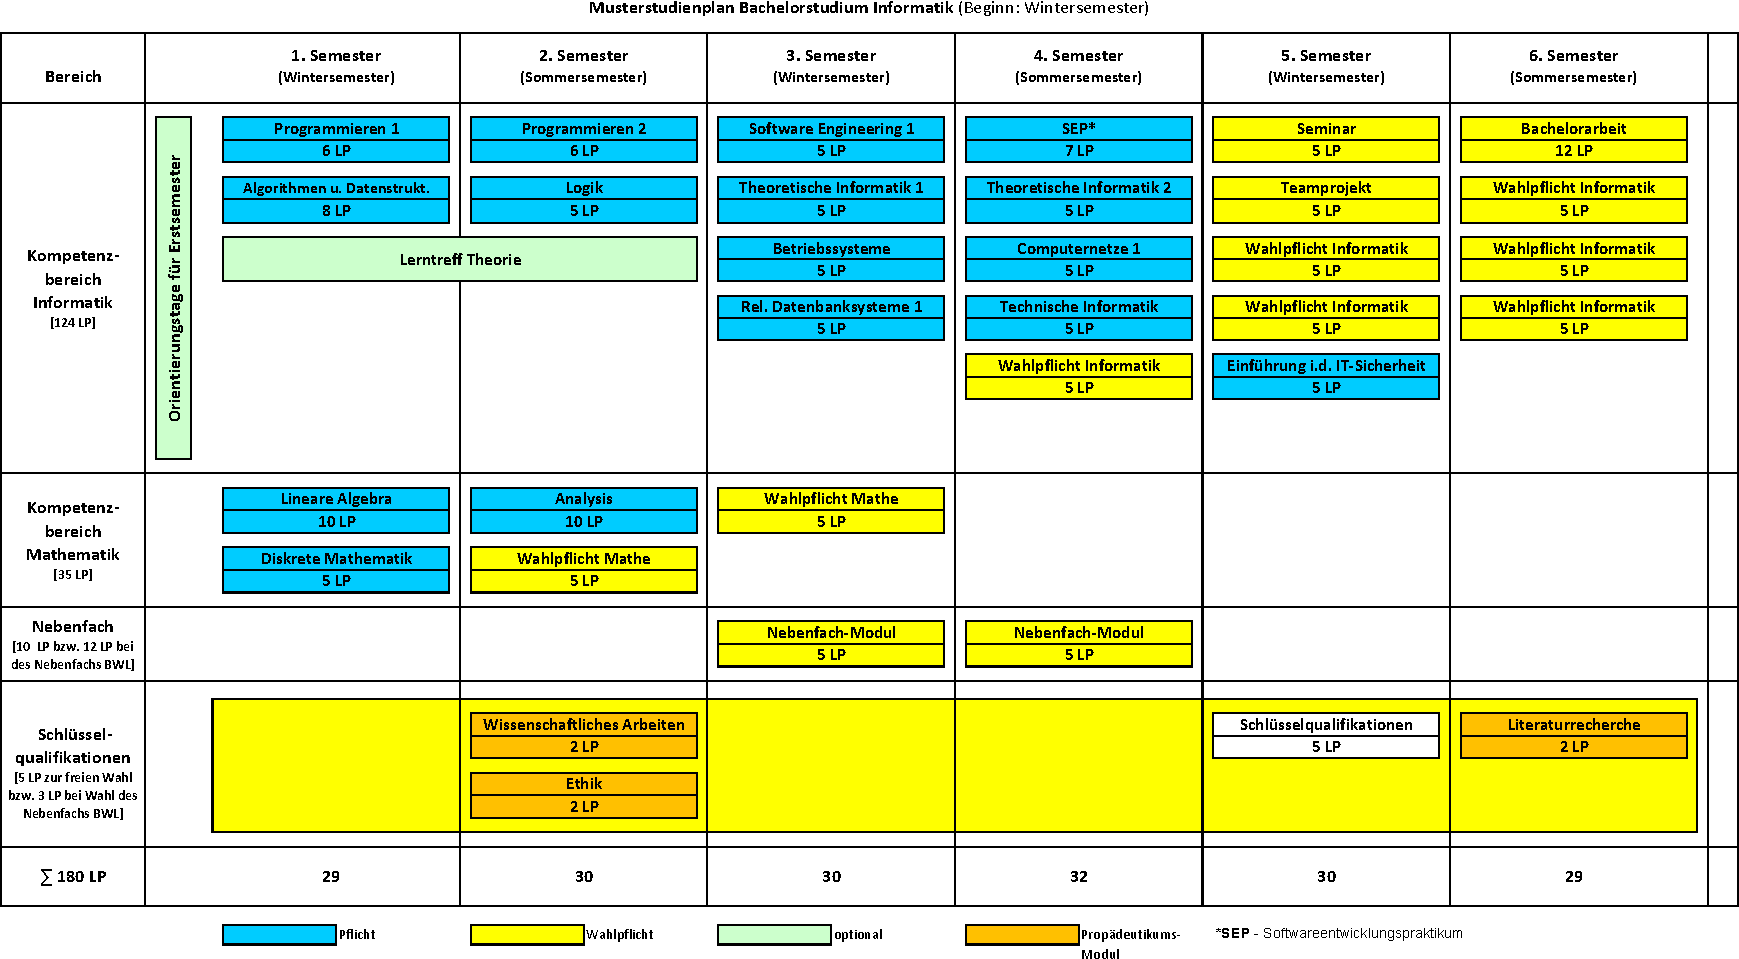
\includegraphics[angle=90, height=\textheight]{bilder/studienplan_bsc/WS-Fak.pdf}
	\end{center}

	\newpage

	\begin{center} 
		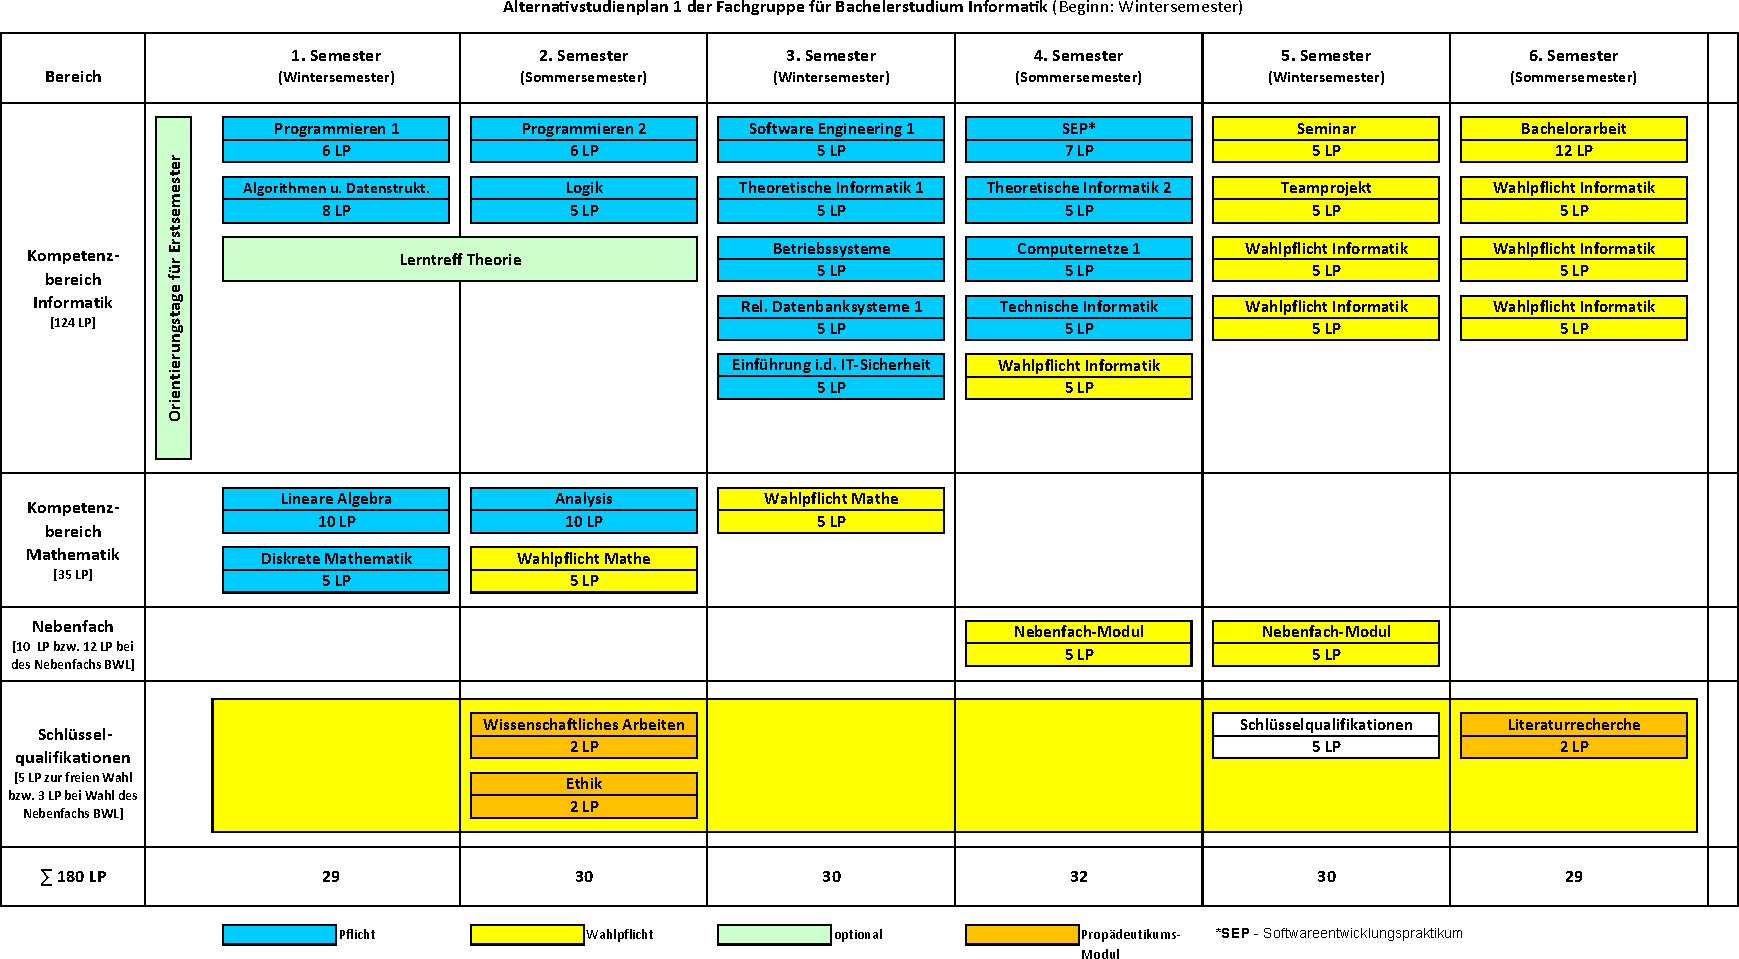
\includegraphics[angle=90, height=\textheight]{bilder/studienplan_bsc/WS-FG-easy.pdf}
	\end{center}

	\newpage

	\begin{center} 
		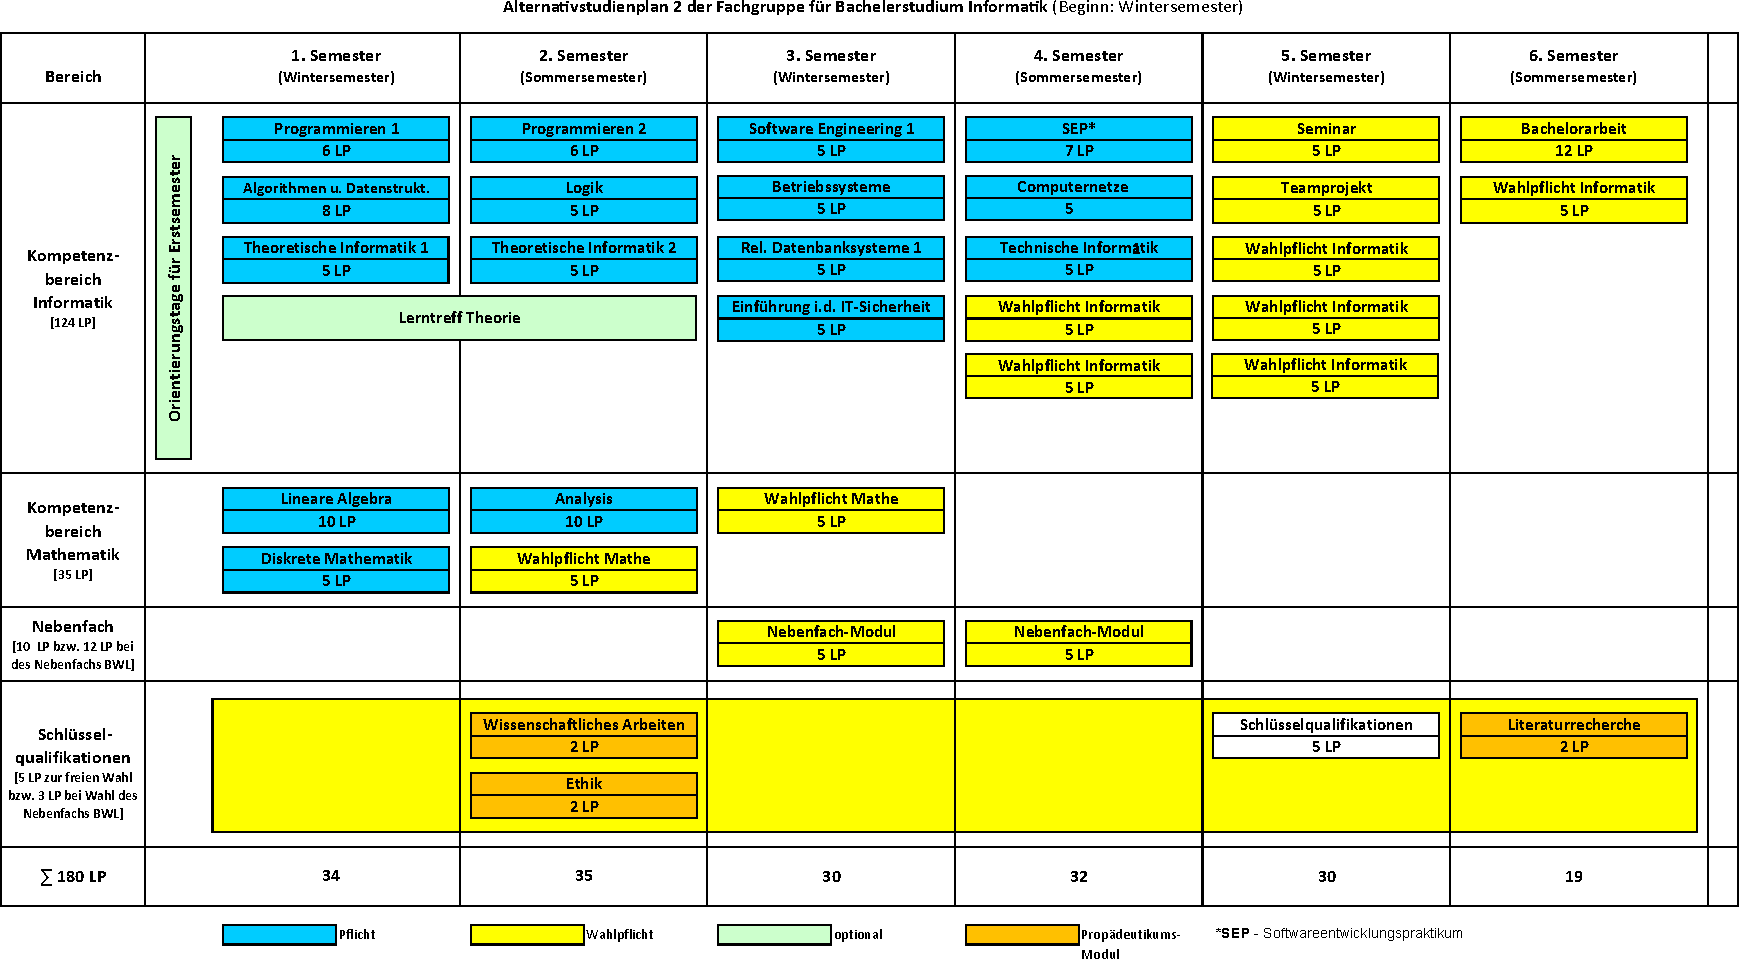
\includegraphics[angle=90, height=\textheight]{bilder/studienplan_bsc/WS-FG-hard.pdf}
	\end{center}
}{
	\tocheck{4}{Aktuelle Musterstudienpläne für SS erzeugen und einpfelgen!}
}
